\subsection{emcee first results}\label{emcee first results}
In this section the first results of emcee are presented. Emcee was used to calibrate four different MODFLOW6 models (\hyperref[fig_logbook_1.0_CONGROMO]{\textcolor{blue}{Figure }\ref{fig_logbook_1.0_CONGROMO}}). 
The main purpose of this section is to check whether the samplers work as intended and to identify possible issues. Three different samplers were compared: Stretch, Differential evolution (DE) and lastly a combination of Differential Evolution (frequency 0.8) \& snooker update (frequency 0.2), which from here on will be referred to as DEsnooker. All three samplers were ran for three ensembles per model, with each ensemble consisting of 10 chains. All chains were run for 500 steps burn-in and an additional 1000 steps of main-sampling. The different samplers were initialised at the same position for fair comparison, with starting positions selected stochastically from Unif(0.0001,20). Priors for all parameters were set to N(10,10) and measurement uncertainty, which determines the likelihood function, was set to N(0,0.1). Ensembles were saved separately in h5 files, resulting in 36 files created.   
%Better subsubsections may be areas of research or problems. So something like convergence to true parameter values OR 

\begin{figure}[H]
\centering
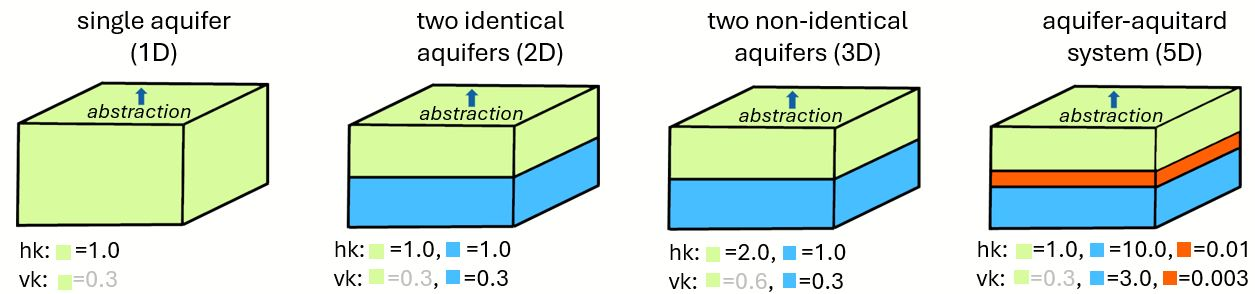
\includegraphics[width=0.9\textwidth]{Figures/appendix_figs/C.1.0 conceptual_groundwater_models_ppt.JPG}
\caption{\textbf{[outdated figure, need to make a new sketch]} Schematic of the four conceptual groundwater flow models designed so far. All conceptual groundwater flow models have a length and width of 1000 meters and a depth of 50 meters. At the centre of each conceptual groundwater flow model is a well, extending over the full depth of the phreatic aquifer, with an extraction rate of 500 m\textsuperscript{3}/day. At the edges of the conceptual groundwater flow models, there are constant head boundaries of 10 meters. In the figure above each conceptual groundwater flow model the number of calibrated parameters is indicated by e.g. 1D, indicating a single parameter to be calibrated. Below each conceptual groundwater flow model the horizontal hydraulic conductivity (hk) and vertical hydraulic conductivity (vk) are given in m/day. Note that for each conceptual groundwater flow model the number of hydraulic conductivities is one higher than the number of calibrated parameters, this is due to the model being insensitive to the vertical conductivity in the phreatic aquifer.}\label{fig_logbook_1.0_CONGROMO} %so the location of the label influences how it is referenced!?, that's clunky
\end{figure}

\subsubsection{trace plots} %Case study of Model 4
Trace plots are presented for model four to investigate whether the different moves explore the parameter space as intended. Model four was selected, because it has the highest number of parameters to be calibrated (5). The ensemble and subsequent chain selection was arbitrary. 

The first 600 steps of the Stretch sampler of a specific chain show little variation in parameter values (\hyperref[fig_logbook_1.1_trace_plot_Stretch]{\textcolor{blue}{Figure }\ref{fig_logbook_1.1_trace_plot_Stretch}}), suggesting high autocorrelation and low acceptance fraction for proposals. This problem appears to be even worse for the DE sampler (\hyperref[fig_logbook_1.1_trace_plot_DE]{\textcolor{blue}{Figure }\ref{fig_logbook_1.1_trace_plot_DE}}) and for the DEsnooker sampler (\hyperref[fig_logbook_1.1_trace_plot_DEsnooker]{\textcolor{blue}{Figure }\ref{fig_logbook_1.1_trace_plot_DEsnooker}}), with the chains moving only roughly every hundred steps. Another problem is that parameter 2 in \hyperref[fig_logbook_1.1_trace_plot_Stretch]{\textcolor{blue}{Figure }\ref{fig_logbook_1.1_trace_plot_Stretch}} appears to never move. 

The acceptance fraction for these specific chains has been calculated to verify whether the chains indeed exhibit the infrequent movement suggested by the trace plots, or if the moves are so small that they are not detectable in the trace plots. The acceptance fraction for different parameter within specific chains does not vary (\hyperref[tab_logbook_1.1_acceptance_frac]{\textcolor{blue}{Table }\ref{tab_logbook_1.1_acceptance_frac}}). Thus, parameter 2 in \hyperref[fig_logbook_1.1_trace_plot_Stretch]{\textcolor{blue}{Figure }\ref{fig_logbook_1.1_trace_plot_Stretch}} does move as intended, but due to the scale it is not visible. All acceptance fractions are low, as was expected based on the trace plots, with DE scoring the worst with roughly 1 in 100 proposals being accepted. These acceptance fractions are very low compared to the ideal acceptance fractions, which, as a rule of thumb, should be between 0.2 and 0.5 \citep{foreman2013emcee}. 


\begin{figure}[H]
\centering
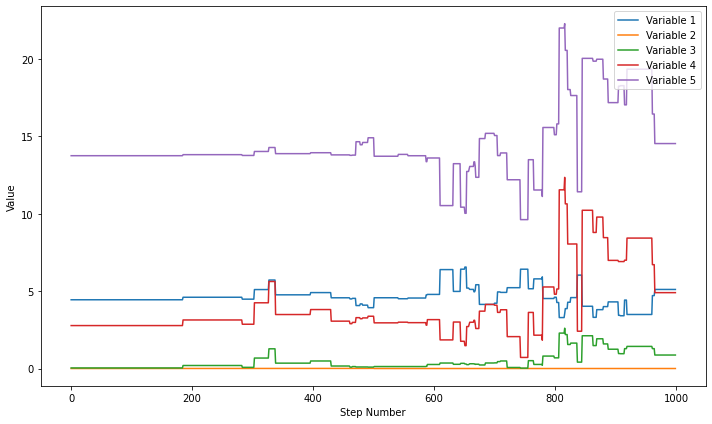
\includegraphics[width=\textwidth]{Figures/appendix_figs/C.1.1 trace plot Stretch.png}
\caption{A trace plot of the Stretch move for calibrating model four. The presented chain is the 2\textsuperscript{nd} chain of the 3\textsuperscript{rd}  ensemble. Only the 1000 steps of the main sampling are presented, the 500 burn-in steps were discarded. }\label{fig_logbook_1.1_trace_plot_Stretch}
\end{figure}

\begin{figure}[ht]
\centering
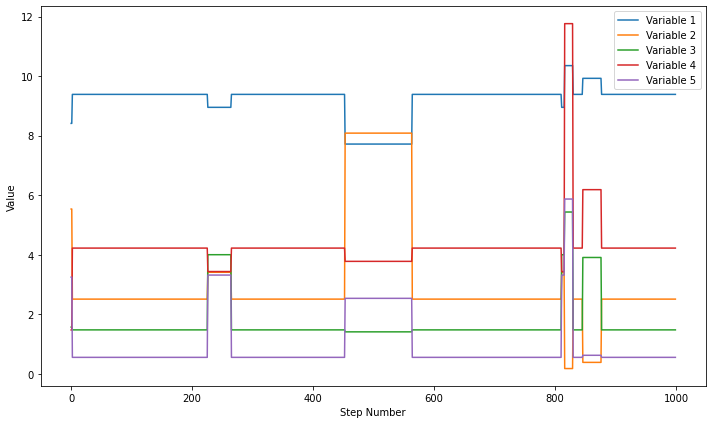
\includegraphics[width=\textwidth]{Figures/appendix_figs/C.1.1 trace plot DE.png}
\caption{A trace plot of the Differential Evolution move for calibrating model four. The presented chain is the 2\textsuperscript{nd}
chain of the 3\textsuperscript{rd} ensemble. Only the 1000 steps of the main sampling are presented, the 500 burn-in steps were discarded.}\label{fig_logbook_1.1_trace_plot_DE}
\end{figure}

\begin{figure}[hb]
\centering
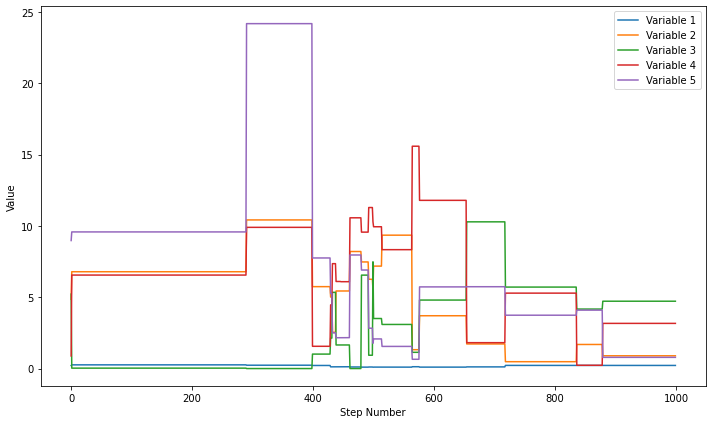
\includegraphics[width=\textwidth]{Figures/appendix_figs/C.1.1 trace plot DEsnooker.png}
\caption{A trace plot of a combination
of Differential Evolution (frequency 0.8) \& snooker update (frequency 0.2) moves for calibrating model four. The presented chain is the 2\textsuperscript{nd}
chain of the 3\textsuperscript{rd} ensemble. Only the 1000 steps of the main sampling are presented, the 500 burn-in steps were discarded.}\label{fig_logbook_1.1_trace_plot_DEsnooker}
\end{figure}

\clearpage % to keep two figures on one page, before the table

\begin{table}[ht]
\centering
\caption{Compares the acceptance fraction of proposed steps by different samplers (Stretch, DE, DEsnooker)  for calibrating Model four. The presented acceptance fractions for each parameter ($\theta$) are from the 2\textsuperscript{nd} chain of the 3\textsuperscript{rd} ensemble of each sampler.}
\label{tab_logbook_1.1_acceptance_frac}
\begin{tabularx}{\textwidth}{XXXXXX}
\toprule
 & \(\theta_1\) & \(\theta_2\) & \(\theta_3\) & \(\theta_4\) & \(\theta_5\) \\
\midrule
Stretch & 0.059 & 0.059 & 0.059 & 0.059 & 0.059 \\
DE & 0.011 & 0.011 & 0.011 & 0.011 & 0.011 \\
DEsnooker & 0.020 & 0.020 & 0.020 & 0.020 & 0.020 \\
\bottomrule
\end{tabularx}
\centering
\end{table}

\subsubsection{convergence}
In the previous section a single chain for a single model was explored. Expanding the scope of analysis, this section will compare all ensembles of all models using various summary statistics. The acceptance fraction of proposals will be computed again, as it was shown to be alarmingly low for the specific chain, analysed in the previous section  (\hyperref[tab_logbook_1.1_acceptance_frac]{\textcolor{blue}{Table }\ref{tab_logbook_1.1_acceptance_frac}}). the The integrated autocorrelation time will be computed ($\hat{\tau}$), which should give some further insight into the efficiency of the different samplers. The new Gelman-Rubin diagnositc ($\hat{R}$), as introduced by \citet{vehtari2021rank}, will be computed to evaluate convergence. Finally the mean ($\mu$) and standard deviation ($\sigma$) of each ensemble will be computed, to determine whether the different samplers converged to the true posterior.   

The mean acceptance fraction of proposals for all ensembles of Model 1, Model 2 and Model 3 ranges between 0.21 and 0.77 (\hyperref[tab_logbook_1.2_acceptance_frac]{\textcolor{blue}{Table }\ref{tab_logbook_1.2_acceptance_frac}}). The mean acceptance fractions of the Stretch move are higher than DE and DEsnooker, but not so high as to risk approaching a drunkards walk, with 0.766 as the highest. The mean acceptance fraction for the first three models also decreases somewhat for higher model numbers. This is ideal as with increasing dimensionality (increases with model number) the optimal value for the mean acceptance fraction decreases \citet{gelman2021bayesian}. Consistency between ensembles looks promising, with different ensembles for the same move and model showing very similar mean acceptance fractions. The standard deviations are relatively small compared to the mean acceptance fractions, which implies little variation between chains. In conclusion, the acceptance fractions of the first 3 models are satisfactory. 

In contrast, the acceptance fractions of Model 4 are so low that the samplers become inefficient (slow exploration and convergence). This is especially the case for DE and DEsnooker with mean acceptance fractions ranging from 0.003 up to 0.024. For the stretch move the mean acceptance fractions are still acceptable. It appears that the chain presented in \hyperref[tab_logbook_1.1_acceptance_frac]{\textcolor{blue}{Table }\ref{tab_logbook_1.1_acceptance_frac}} is not representative of the mean acceptance fraction, but more of a lower extreme. 

The integrated autocorrelation time ($\hat{\tau}$) is consistently higher for the Stretch move than for DE and DEsnooker, with the exception of Model 4 (\hyperref[tab_logbook_1.2_tau]{\textcolor{blue}{Table }\ref{tab_logbook_1.2_tau}}). Although more proposals are accepted by the Stretch move (\hyperref[tab_logbook_1.2_acceptance_frac]{\textcolor{blue}{Table }\ref{tab_logbook_1.2_acceptance_frac}}), the proposals are more correlated than for DE and DEsnooker (\hyperref[tab_logbook_1.2_tau]{\textcolor{blue}{Table }\ref{tab_logbook_1.2_tau}}). This implies that the performane of the Stretch move is actually the lowest out of all three moves for Model 1-3. The reported standard deviations of all moves are relatively small with respect to the mean for Model 1-3, implying little difference between parameters. 

For Model 4 it was not possible to calculate $\hat{\tau}$ for every ensemble of DE and DEsnooker, perhaps due to the very low acceptance fraction of these ensembles. The mean $\hat{\tau}$ values of Model 4 that could be computed show little variation between the samplers.    

\textbf{Alarmingly}, $\hat{\tau}$ of ensemble 2 of DE for Model 4 reports a mean value of 74, which is higher than 1/acceptance fraction. This should not be possible, as this would require better than independent sampling, which is theoretically impossible. Hopefully this is a result of using too short chains to accurately compute $\hat{\tau}$. 

\begin{table}[ht]
\caption{Acceptance fraction of proposed steps by different samplers (Stretch, DE, DEsnooker), with each three ensembles (e), for calibrating four different models. For each ensemble, the mean acceptance fraction and its standard deviation are presented in the format: mean (std).}
\label{tab_logbook_1.2_acceptance_frac}
\begin{tabularx}{\textwidth}{XXXXX}
\toprule
 & Model 1 & Model 2 & Model 3 & Model 4 \\
\midrule
Stretch (e1) & 0.766 (0.047) & 0.625 (0.020) & 0.571 (0.030) & 0.142 (0.045) \\
Stretch (e2) & 0.737 (0.095) & 0.639 (0.034) & 0.575 (0.028) & 0.169 (0.062) \\
Stretch (e3) & 0.752 (0.043) & 0.620 (0.019) & 0.571 (0.033) & 0.123 (0.053) \\
\midrule
DE (e1) & 0.399 (0.016) & 0.254 (0.016) & 0.227 (0.019) & 0.009 (0.005) \\
DE (e2) & 0.395 (0.028) & 0.293 (0.016) & 0.258 (0.012) & 0.014 (0.008) \\
DE (e3) & 0.421 (0.014) & 0.277 (0.022) & 0.258 (0.020) & 0.003 (0.004) \\
\midrule
DEsnooker (e1) & 0.339 (0.016) & 0.277 (0.011) & 0.226 (0.021) & 0.013 (0.007) \\
DEsnooker (e2) & 0.335 (0.016) & 0.262 (0.009) & 0.217 (0.008) & 0.015 (0.008) \\
DEsnooker (e3) & 0.365 (0.020) & 0.276 (0.015) & 0.210 (0.014) & 0.024 (0.014) \\
\bottomrule
\end{tabularx}
\end{table}

\begin{table}[ht]
\caption{Estimated integrated autocorrelation time ($\hat{\tau}$) of different samplers (Stretch, DE, DEsnooker), with each three ensembles (e), for calibrating four different models. For each parameter in the ensemble only one value for $\hat{\tau}$ is computed. The mean $\hat{\tau}$ of all parameters and the standard deviation are presented in the format: mean (std).}
\label{tab_logbook_1.2_tau}
\begin{tabularx}{\textwidth}{XXXXX}
\toprule
 & Model 1 & Model 2 & Model 3 & Model 4 \\
\midrule
Stretch (e1) & 28 (0.0) & 35 (0.8) & 43 (4.2) & 90 (6.5) \\
Stretch (e2) & 38 (0.0) & 39 (0.5) & 38 (4.6) & 95 (6.0) \\
Stretch (e3) & 39 (0.0) & 38 (0.4) & 43 (2.3) & 92 (11.1) \\
\midrule
DE (e1) & \phantom{0}9 (0.0) & 21 (4.7) & 22 (4.9) & 74 (12.6) \\
DE (e2) & 13 (0.0) & 11 (2.4) & 14 (2.0) & 96 (6.3) \\
DE (e3) & \phantom{0}8 (0.0) & 16 (2.8) & 15 (3.4) & nan (nan) \\
\midrule
DEsnooker (e1) & 12 (0.0) & 17 (4.4) & 16 (1.7) & nan (nan) \\
DEsnooker (e2) & 15 (0.0) & 23 (3.8) & 18 (1.1) & nan (nan) \\
DEsnooker (e3) & 10 (0.0) & 22 (3.7) & 16 (2.9) & 101 (4.8) \\
\bottomrule
\end{tabularx}
\end{table}

The Gelman-Rubin diagnostic ($\hat{R}$) of all ensembles is 1.01 or higher (\hyperref[tab_logbook_1.2_rhat]{\textcolor{blue}{Table }\ref{tab_logbook_1.2_rhat}}), indicating that none of the ensembles have converged \cite{vehtari2021rank}. The Stretch move has higher $\hat{R}$ values for Model 1-3, which is in agreement with the relatively high $\hat{\tau}$ values for the Stretch move (\hyperref[tab_logbook_1.2_tau]{\textcolor{blue}{Table }\ref{tab_logbook_1.2_tau}}). For Model 4 both $\hat{R}$ and $\hat{\tau}$ are again consistent, both reporting very high values for all moves. 

\begin{table}[ht]
\caption{Gelman-Rubin diagnostic ($\hat{R}$) of different samplers (Stretch, DE, DEsnooker), with each three ensembles (e), for calibrating four different models. For each parameter in the ensemble only one value for $\hat{R}$ is computed. The mean $\hat{R}$ of all parameters and the standard deviation are presented in the format: mean (std).}
\label{tab_logbook_1.2_rhat}
\begin{tabularx}{\textwidth}{XXXXX}
\toprule
 & Model 1 & Model 2 & Model 3 & Model 4 \\
\midrule
Stretch (e1) & 1.06 (0.000) & 1.10 (0.003) & 1.06 (0.016) & 2.14 (0.393) \\
Stretch (e2) & 1.09 (0.000) & 1.08 (0.000) & 1.06 (0.023) & 1.78 (0.407) \\
Stretch (e3) & 1.04 (0.000) & 1.07 (0.004) & 1.05 (0.021) & 2.44 (0.308) \\
\midrule
DE (e1) & 1.01 (0.000) & 1.04 (0.003) & 1.03 (0.017) & 2.66 (0.523) \\
DE (e2) & 1.01 (0.000) & 1.02 (0.002) & 1.02 (0.007) & 2.01 (0.237) \\
DE (e3) & 1.01 (0.000) & 1.03 (0.006) & 1.02 (0.004) & 7.18 (2.791) \\
\midrule
DEsnooker (e1) & 1.02 (0.000) & 1.02 (0.003) & 1.02 (0.006) & 2.14 (0.230) \\
DEsnooker (e2) & 1.02 (0.000) & 1.03 (0.002) & 1.02 (0.002) & 1.89 (0.159) \\
DEsnooker (e3) & 1.01 (0.000) & 1.01 (0.002) & 1.02 (0.003) & 1.75 (0.111) \\
\bottomrule
\end{tabularx}
\end{table}

\subsubsection{ensemble mean and standard deviation}
For Model 1, the different samplers converge to an ensemble mean of $\theta_1 \sim 20$, which is much larger than the true value of 5.0 (\hyperref[tab_logbook_1.2_rhat]{\textcolor{blue}{Table }\ref{tab_logbook_1.2_mean1}}).
For Model 2 and Model 3, $\theta_1$ appears to be converging to the true value (\hyperref[tab_logbook_1.2_rhat]{\textcolor{blue}{Table }\ref{tab_logbook_1.2_mean2}} and \hyperref[tab_logbook_1.2_rhat]{\textcolor{blue}{Table }\ref{tab_logbook_1.2_mean3}}). However, the other parameters in these two models are far from the true values. 
Also for Model 4 most mean values are far off from the true values (\hyperref[tab_logbook_1.2_rhat]{\textcolor{blue}{Table }\ref{tab_logbook_1.2_mean4}}). Additionally, the standard deviation of the ensemble mean is relatively large compared to the other Models. 

Considering that $\hat{R}$ values for Model 1-3 are $<1.1$, implies that the different samplers are close to convergence. This suggests the existence of different (and stronger) optima than the true values. The artificially added noise (as a proxy for measurement error) is thought to have resulted in shifted optima. This raises the question whether too much noise has been added. 

Alternatively too few observations may have been used for calculating the likelihood. Especially for Model 4, as fewer observations (3) were used than parameters (5). This may have resulted in equifinality, considering the large standard deviation on several parameters for Model 4. For Model 1-3 equifinality is not expected to be the problem, instead the optimum may have shifted. Increasing the number of observations may be a solution here as well, as it will make it less likely for the optimum to shift

\begin{table}[ht]
\caption{Ensemble mean ($\mu$) and the standard deviation of the ensemble mean ($\sigma$), presented as mean (std). Results are from calibrating the parameter ($\theta$) of Model 1 with different samplers (Stretch, DE, DEsnooker), with each three ensembles (e).}
\label{tab_logbook_1.2_mean1}
\begin{tabularx}{\textwidth}{XX}
\toprule
 & $\theta_1$ \\
\midrule
Stretch (e1) & 19.4 (1.8) \\
Stretch (e2) & 19.0 (3.0) \\
Stretch (e3) & 19.3 (1.9) \\
\midrule
DE (e1) & 19.2 (0.4) \\
DE (e2) & 19.3 (1.2) \\
DE (e3) & 19.7 (0.7) \\
\midrule
DEsnooker (e1) & 19.5 (0.8) \\
DEsnooker (e2) & 19.2 (1.0) \\
DEsnooker (e3) & 19.6 (0.5) \\
\midrule
\textbf{True value} & \textbf{5.0} \\
\bottomrule
\end{tabularx}
\end{table}

\begin{table}[ht]
\caption{Ensemble mean ($\mu$) and the standard deviation of the ensemble mean ($\sigma$), presented as mean (std). Results are from calibrating the parameters ($\theta$) of Model 2 with different samplers (Stretch, DE, DEsnooker), with each three ensembles (e).}
\label{tab_logbook_1.2_mean2}
\begin{tabularx}{\textwidth}{XXX}
\toprule
 & $\theta_1$ & $\theta_2$ \\
\midrule
Stretch (e1) & 2.0 (0.3) & 2.3 (0.7) \\
Stretch (e2) & 2.0 (0.3) & 2.2 (0.8) \\
Stretch (e3) & 1.9 (0.3) & 2.4 (0.7) \\
\midrule
DE (e1) & 1.8 (0.2) & 2.6 (0.8) \\
DE (e2) & 1.9 (0.2) & 2.1 (0.2) \\
DE (e3) & 1.9 (0.1) & 2.3 (0.5) \\
\midrule
DEsnooker (e1) & 2.0 (0.1) & 2.1 (0.1) \\
DEsnooker (e2) & 2.0 (0.2) & 2.2 (0.3) \\
DEsnooker (e3) & 1.9 (0.1) & 2.2 (0.3) \\
\midrule
\textbf{True value} & \textbf{2.0} & \textbf{1.0} \\
\bottomrule
\end{tabularx}
\end{table}

\begin{table}[ht]
\caption{Ensemble mean ($\mu$) and the standard deviation of the ensemble mean ($\sigma$), presented as mean (std). Results are from calibrating the parameters ($\theta$) of Model 3 with different samplers (Stretch, DE, DEsnooker), with each three ensembles (e).}
\label{tab_logbook_1.2_mean3}
\begin{tabularx}{\textwidth}{XXXX}
\toprule
 & $\theta_1$ & $\theta_2$ & $\theta_3$ \\
\midrule
Stretch (e1) & 1.5 (0.2) & 9.1 (1.5) & 0.9 (0.1) \\
Stretch (e2) & 1.5 (0.2) & 8.7 (1.1) & 0.9 (0.2) \\
Stretch (e3) & 1.5 (0.1) & 9.1 (1.7) & 1.0 (0.1) \\
\midrule
DE (e1) & 1.5 (0.1) & 9.3 (0.8) & 0.9 (0.2) \\
DE (e2) & 1.5 (0.1) & 9.1 (0.5) & 0.9 (0.1) \\
DE (e3) & 1.4 (0.1) & 9.5 (0.8) & 1.0 (0.1) \\
\midrule
DEsnooker (e1) & 1.4 (0.1) & 9.2 (0.8) & 0.9 (0.1) \\
DEsnooker (e2) & 1.4 (0.1) & 9.7 (0.8) & 0.9 (0.1) \\
DEsnooker (e3) & 1.4 (0.1) & 9.2 (0.6) & 1.0 (0.1) \\
\midrule
\textbf{True value} & \textbf{1.0} & \textbf{0.01} & \textbf{10.0} \\
\bottomrule
\end{tabularx}
\end{table}

\clearpage

\begin{table}[ht]
\caption{Ensemble mean ($\mu$) and the standard deviation of the ensemble mean ($\sigma$), presented as mean (std). Results are from calibrating the parameters ($\theta$) of Model 4 with different samplers (Stretch, DE, DEsnooker), with each three ensembles (e).}
\label{tab_logbook_1.2_mean4}
\begin{tabularx}{\textwidth}{lXXXXX}
\toprule
 & $\theta_1$ & $\theta_2$ & $\theta_3$ & $\theta_4$ & $\theta_5$ \\
\midrule
Stretch (e1) & 0.9 (0.9) & 4.3 (5.2) & 13.6 (7.5) & 11.3 (5.8) & 5.4 (3.4) \\
Stretch (e2) & 1.1 (1.7) & 5.9 (4.3) & 5.6 (2.7) & 5.4 (2.3) & 4.1 (2.8) \\
Stretch (e3) & 1.8 (1.9) & 6.2 (6.6) & 5.0 (5.8) & 11.7 (6.6) & 11.4 (5.2) \\
\midrule
DE (e1) & 1.0 (0.9) & 5.8 (6.9) & 7.0 (10.3) & 9.8 (9.8) & 5.7 (2.2) \\
DE (e2) & 0.6 (0.7) & 5.6 (5.9) & 5.4 (4.9) & 10.4 (8.4) & 5.7 (7.0) \\
DE (e3) & 1.6 (2.6) & 8.9 (10.3) & 8.2 (7.6) & 6.5 (6.2) & 10.3 (12.5) \\
\midrule
DEsnooker (e1) & 0.6 (0.5) & 4.4 (3.0) & 4.8 (3.6) & 7.3 (4.9) & 2.3 (1.3) \\
DEsnooker (e2) & 1.4 (2.6) & 5.0 (6.2) & 4.7 (3.6) & 8.3 (4.1) & 4.1 (4.1) \\
DEsnooker (e3) & 0.6 (0.9) & 5.8 (3.6) & 2.7 (1.8) & 10.5 (5.6) & 5.2 (4.2) \\
\midrule
\textbf{True value} & \textbf{1.0} & \textbf{0.1} & \textbf{4.0} & \textbf{0.01} & \textbf{3.0} \\
\bottomrule
\end{tabularx}
\end{table}

\subsubsection{multimodality}
Model 1-3 show clear unimodal optima for every parameter (\hyperref[fig_logbook_1.4_corner_model1]{\textcolor{blue}{Figure }\ref{fig_logbook_1.4_corner_model1}}, \hyperref[fig_logbook_1.4_corner_model2]{\textcolor{blue}{Figure }\ref{fig_logbook_1.4_corner_model2}} and \hyperref[fig_logbook_1.4_corner_model3]{\textcolor{blue}{Figure }\ref{fig_logbook_1.4_corner_model3}} respectively). Model 4 is clearly multimodal, with the strongest optima close to zero for most parameters and many weaker local optima spread through parameter space (\hyperref[fig_logbook_1.4_corner_model4]{\textcolor{blue}{Figure }\ref{fig_logbook_1.4_corner_model4}}). Apart from small concentrated areas of posterior density, some parameters in Model 4 also show covariance along straight lines. A pair plot was created for Model 4, as an alternative to the corner plot. While the pair plot clearly illustrates the covariance along these lines, it does not effectively highlight the areas of highest posterior density (see \hyperref[fig_logbook_1.4_pair_model4]{\textcolor{blue}{Figure }\ref{fig_logbook_1.4_pair_model4}}). Consequently, corner plots are preferred over pair plots for this analysis."
% show pair and or corner plots
% plot vertical lines with true values (for future plots)


\begin{figure}[ht]
\centering
\begin{minipage}[b]{0.45\textwidth}
    \centering
    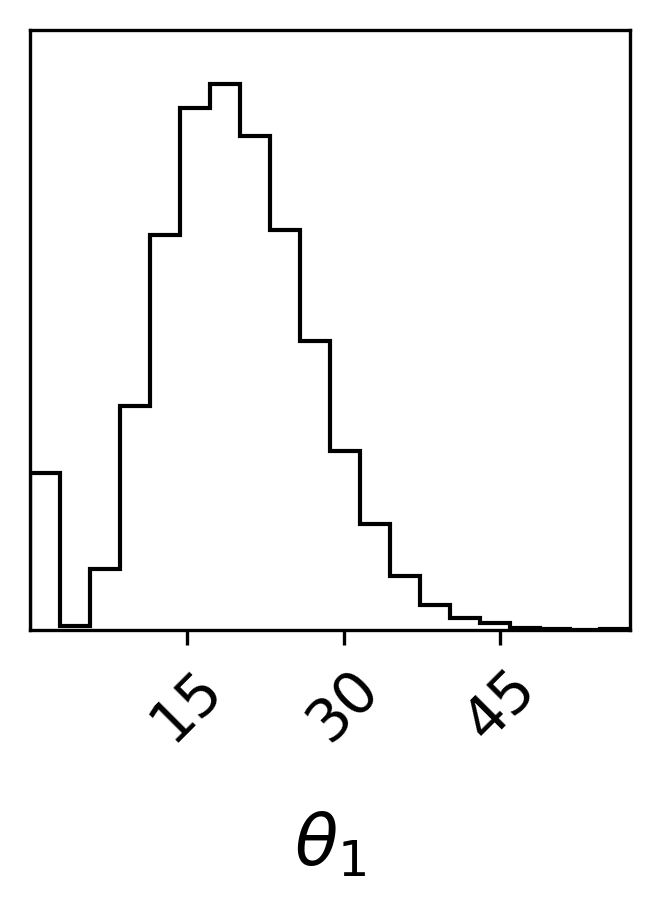
\includegraphics[width=\textwidth]{Figures/appendix_figs/C1.4 corner plot Model 1.png}
    \caption{A corner plot of parameter ($\sigma_1$) of Model 1. All chains of all ensembles of all samplers (Stretch, DE and DEsnooker) were used to create this figure. Darker shades indicate areas of higher posterior density.}\label{fig_logbook_1.4_corner_model1}
\end{minipage}
\hfill
\begin{minipage}[b]{0.45\textwidth}
    \centering
    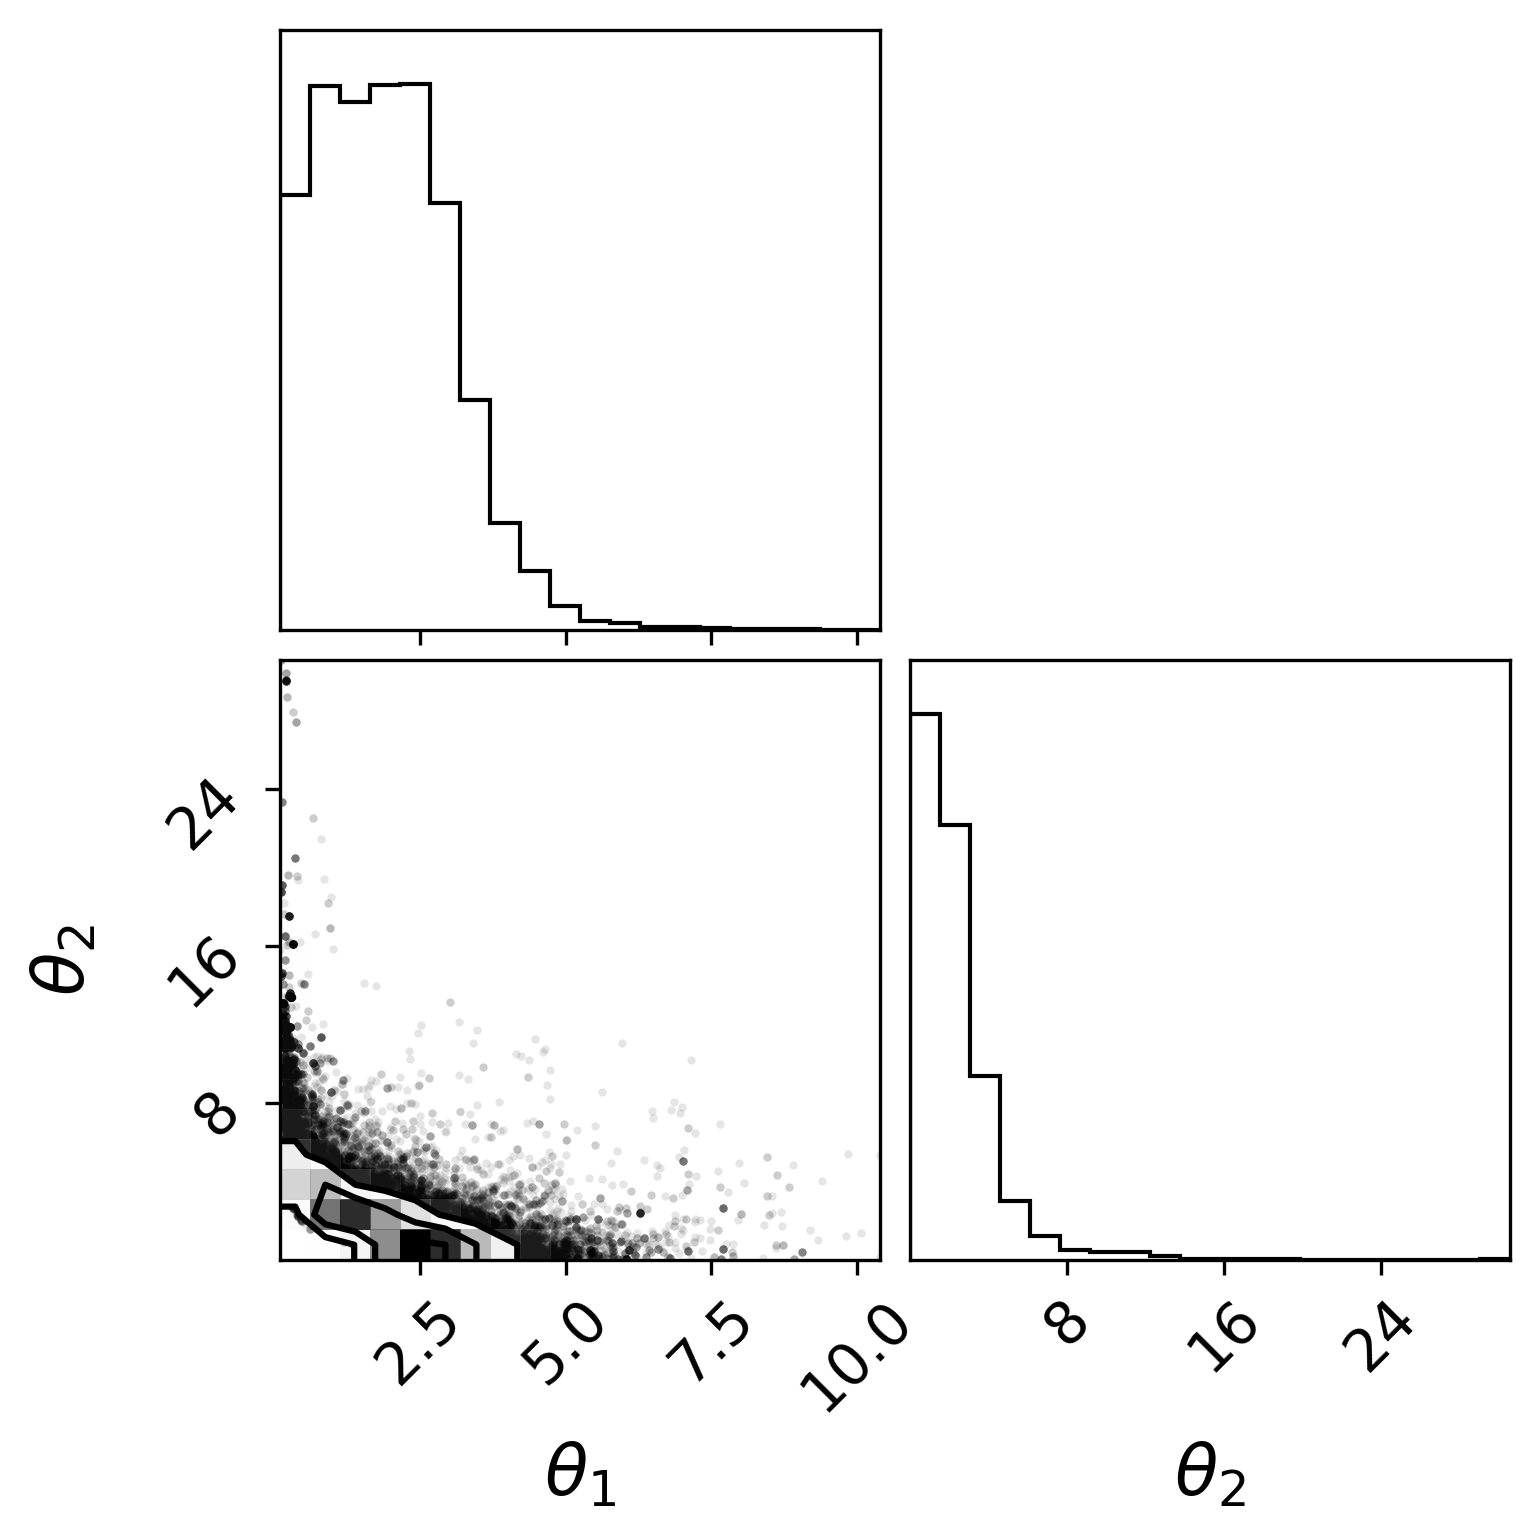
\includegraphics[width=\textwidth]{Figures/appendix_figs/C1.4 corner plot Model 2.png}
    \caption{A corner plot of the parameters ($\sigma$) of Model 2. All chains of all ensembles of all samplers (Stretch, DE and DEsnooker) were used to create this figure. Darker shades indicate areas of higher posterior density.}\label{fig_logbook_1.4_corner_model2}
\end{minipage}
\end{figure}

\begin{figure}[ht]
\centering
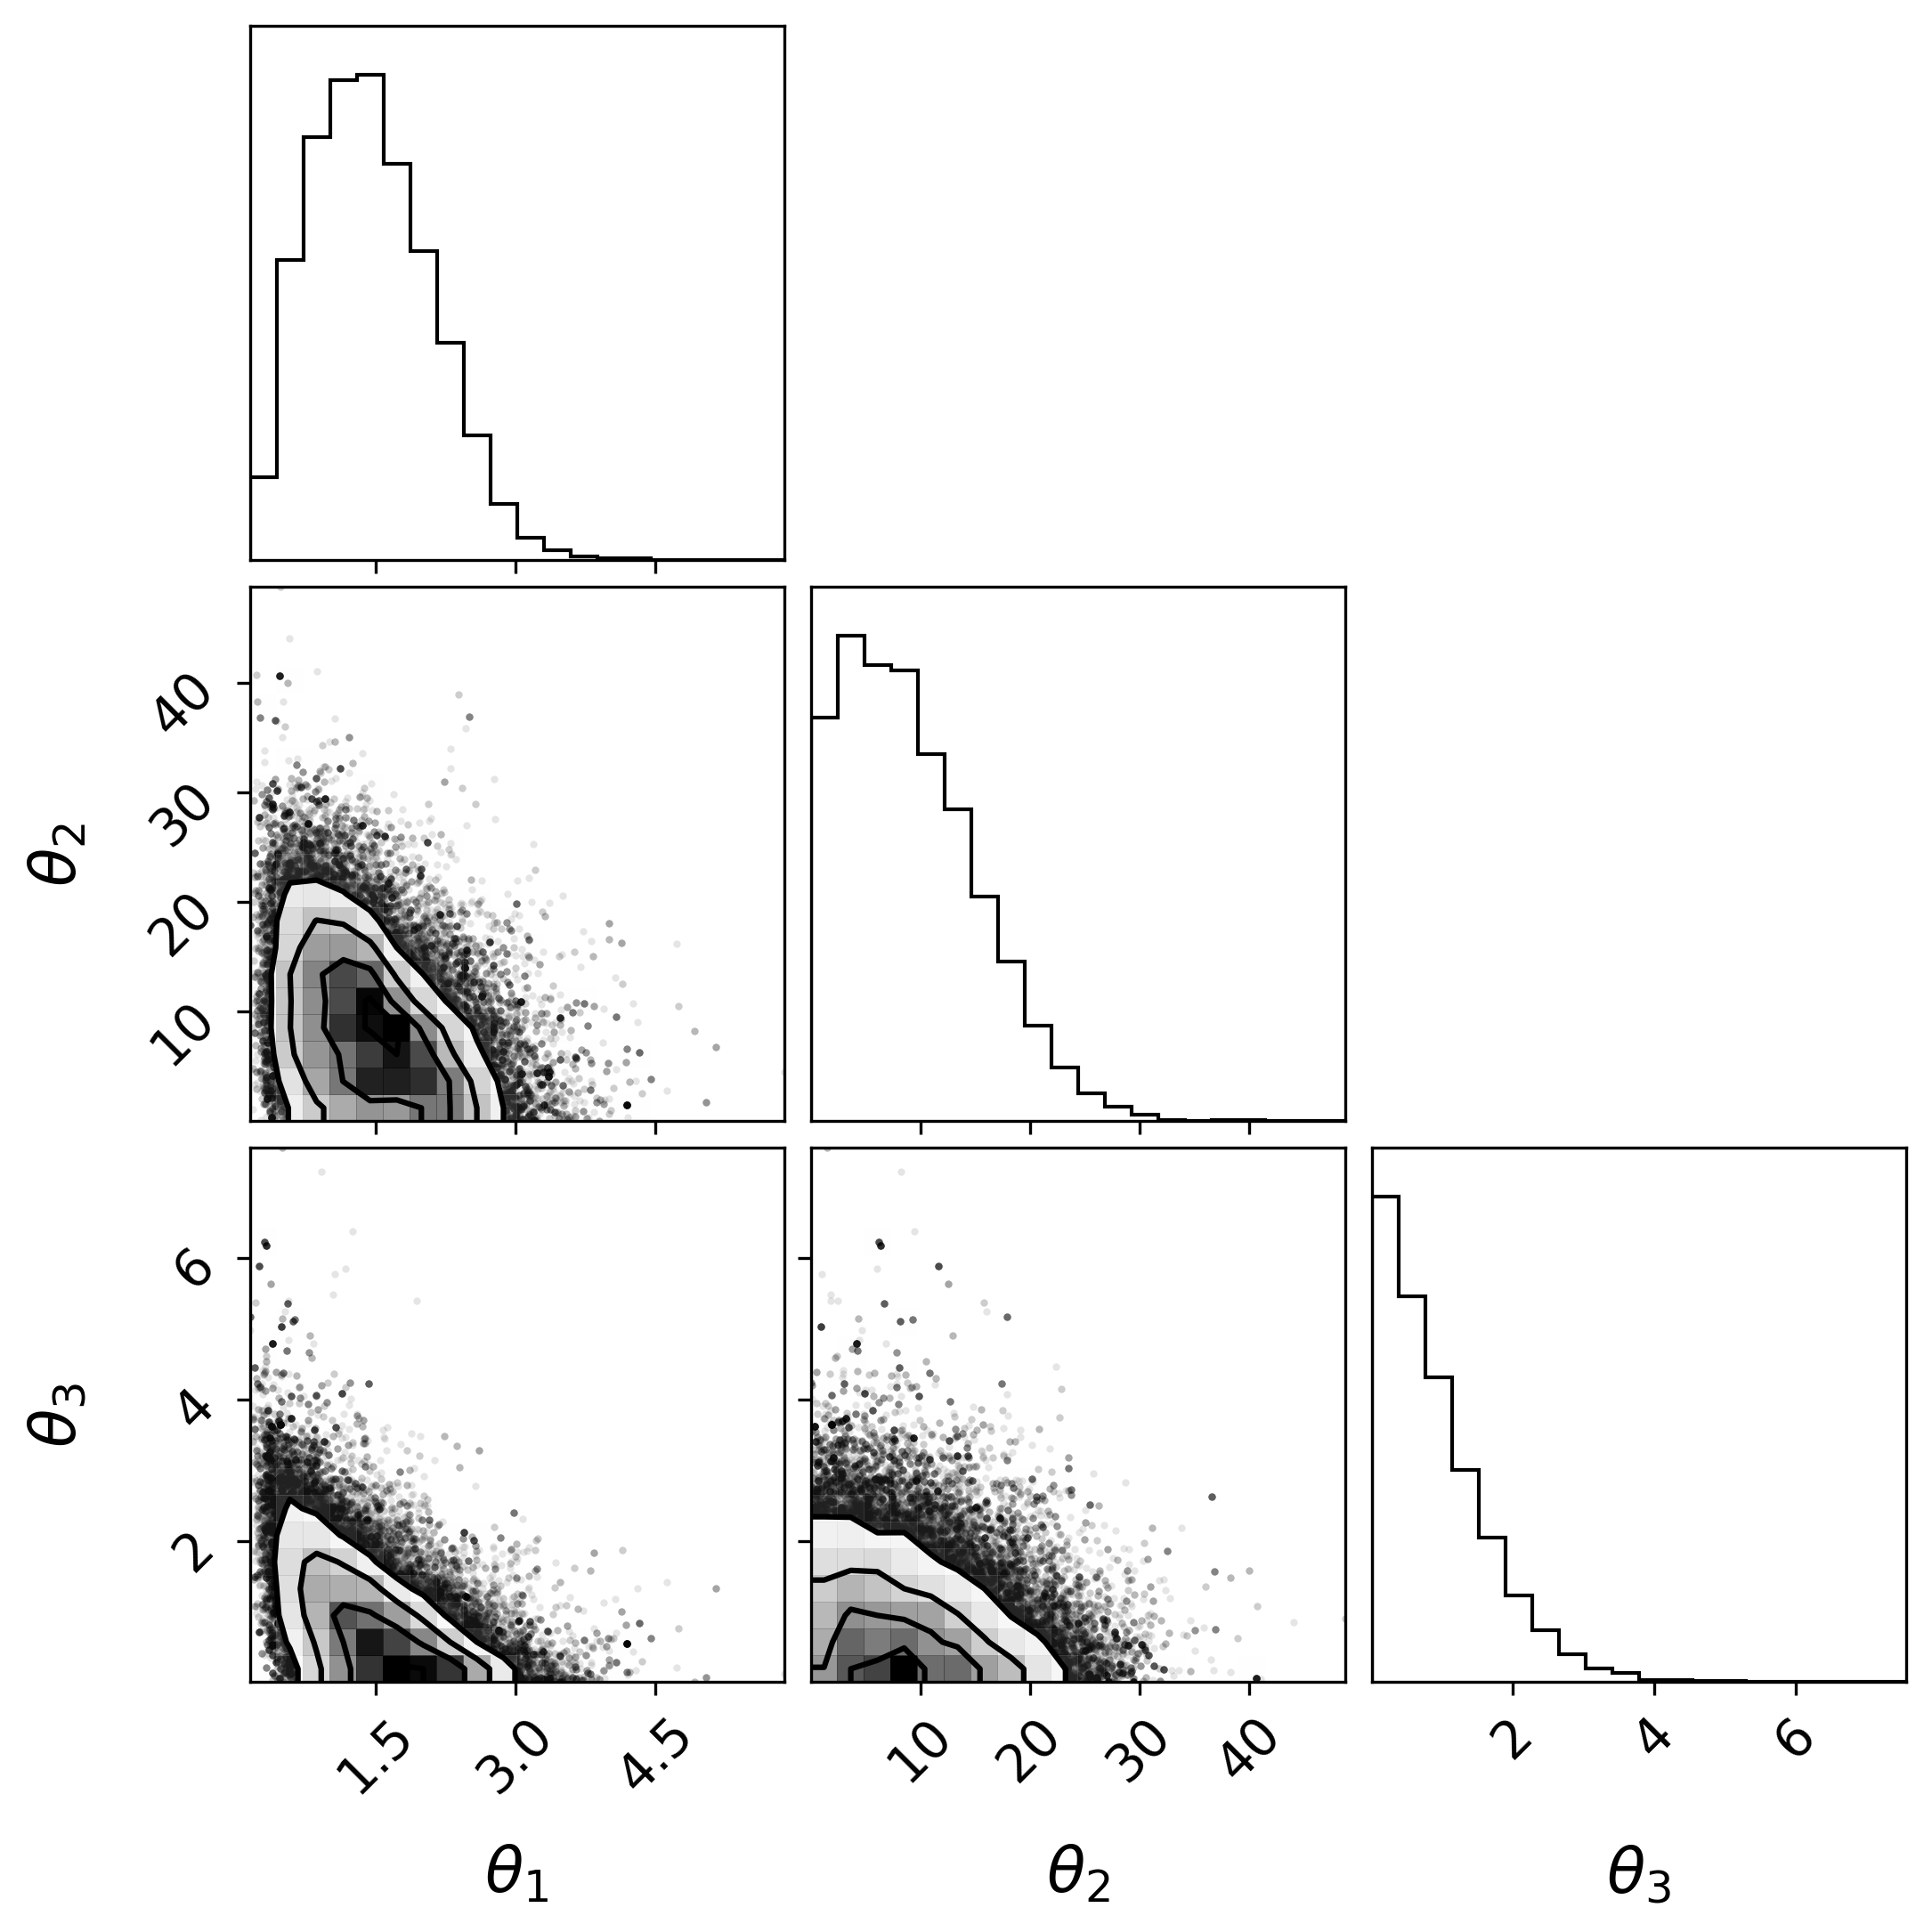
\includegraphics[width=\textwidth]{Figures/appendix_figs/C1.4 corner plot Model 3.png}
\caption{A corner plot of the parameters ($\sigma$) of Model 3. All chains of all ensembles of all samplers (Stretch, DE and DEsnooker) were used to create this figure. Darker shades indicate areas of higher posterior density.}\label{fig_logbook_1.4_corner_model3}
\end{figure}

\begin{figure}[ht]
\centering
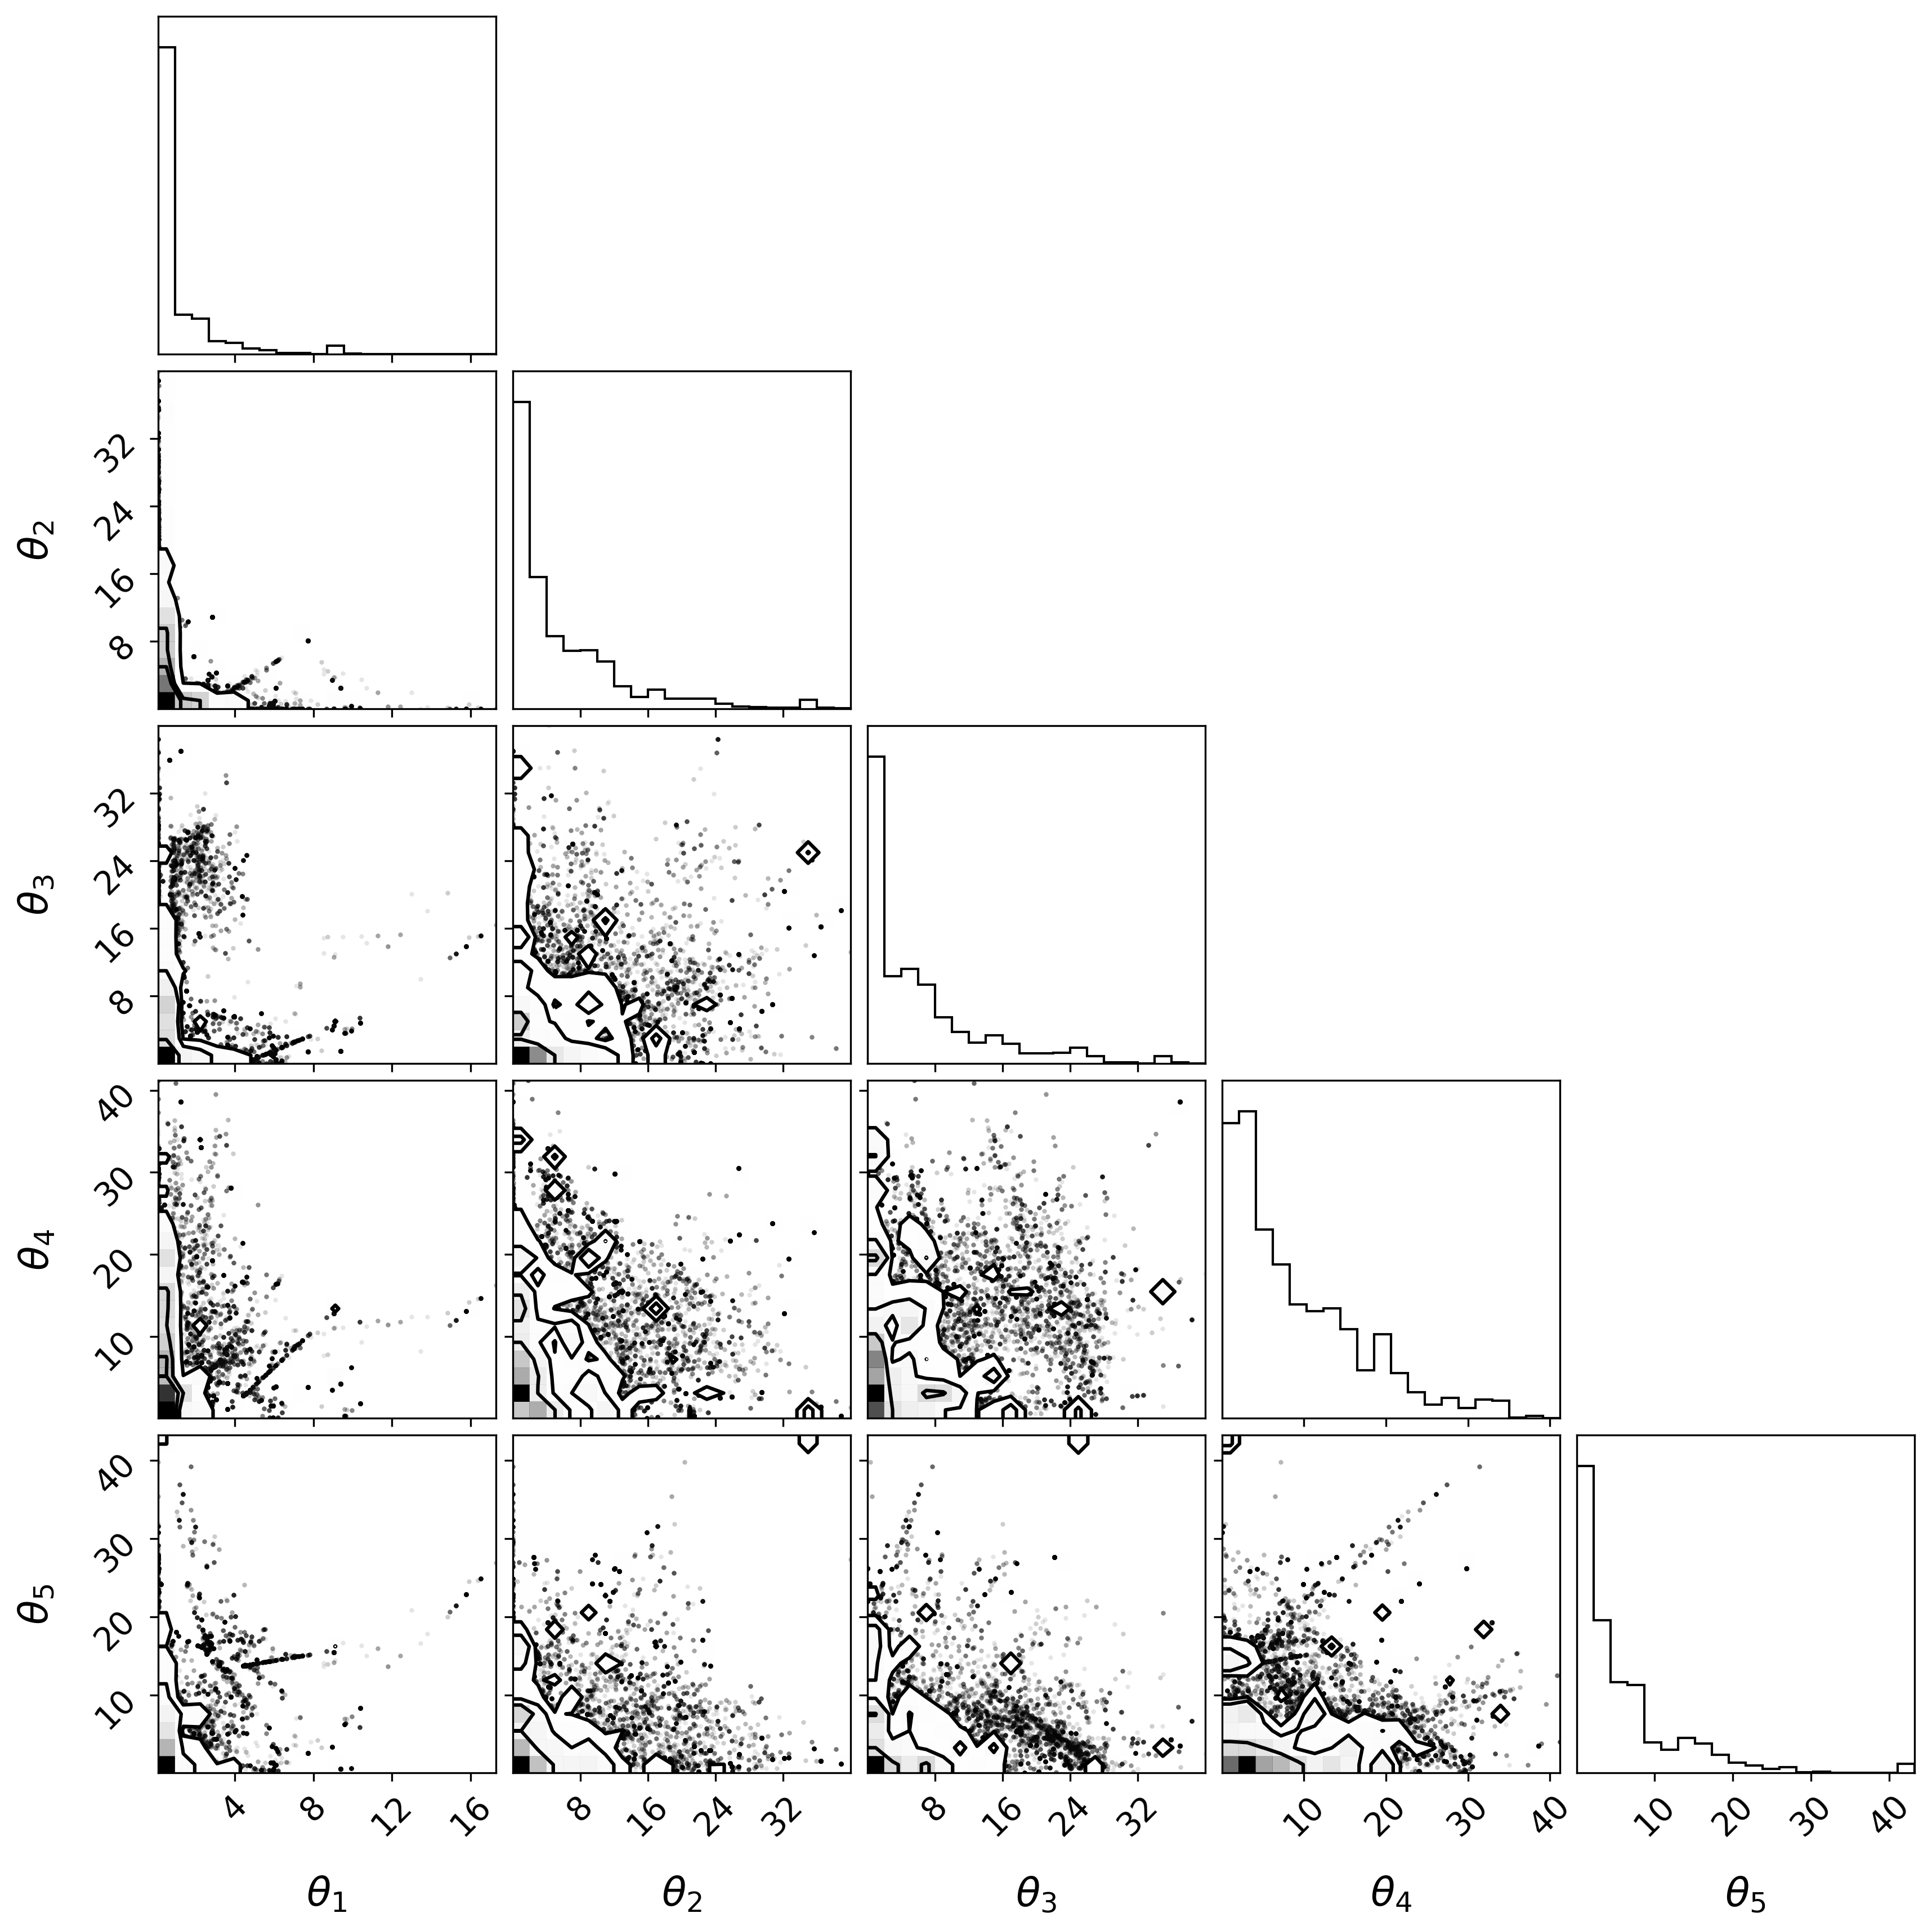
\includegraphics[width=\textwidth]{Figures/appendix_figs/C1.4 corner plot Model 4.png}
\caption{A corner plot of the parameters ($\sigma$) of Model 4. All chains of all ensembles of all samplers (Stretch, DE and DEsnooker) were used to create this figure. Darker shades indicate areas of higher posterior density.}\label{fig_logbook_1.4_corner_model4}
\end{figure}

\begin{figure}[ht]
\centering
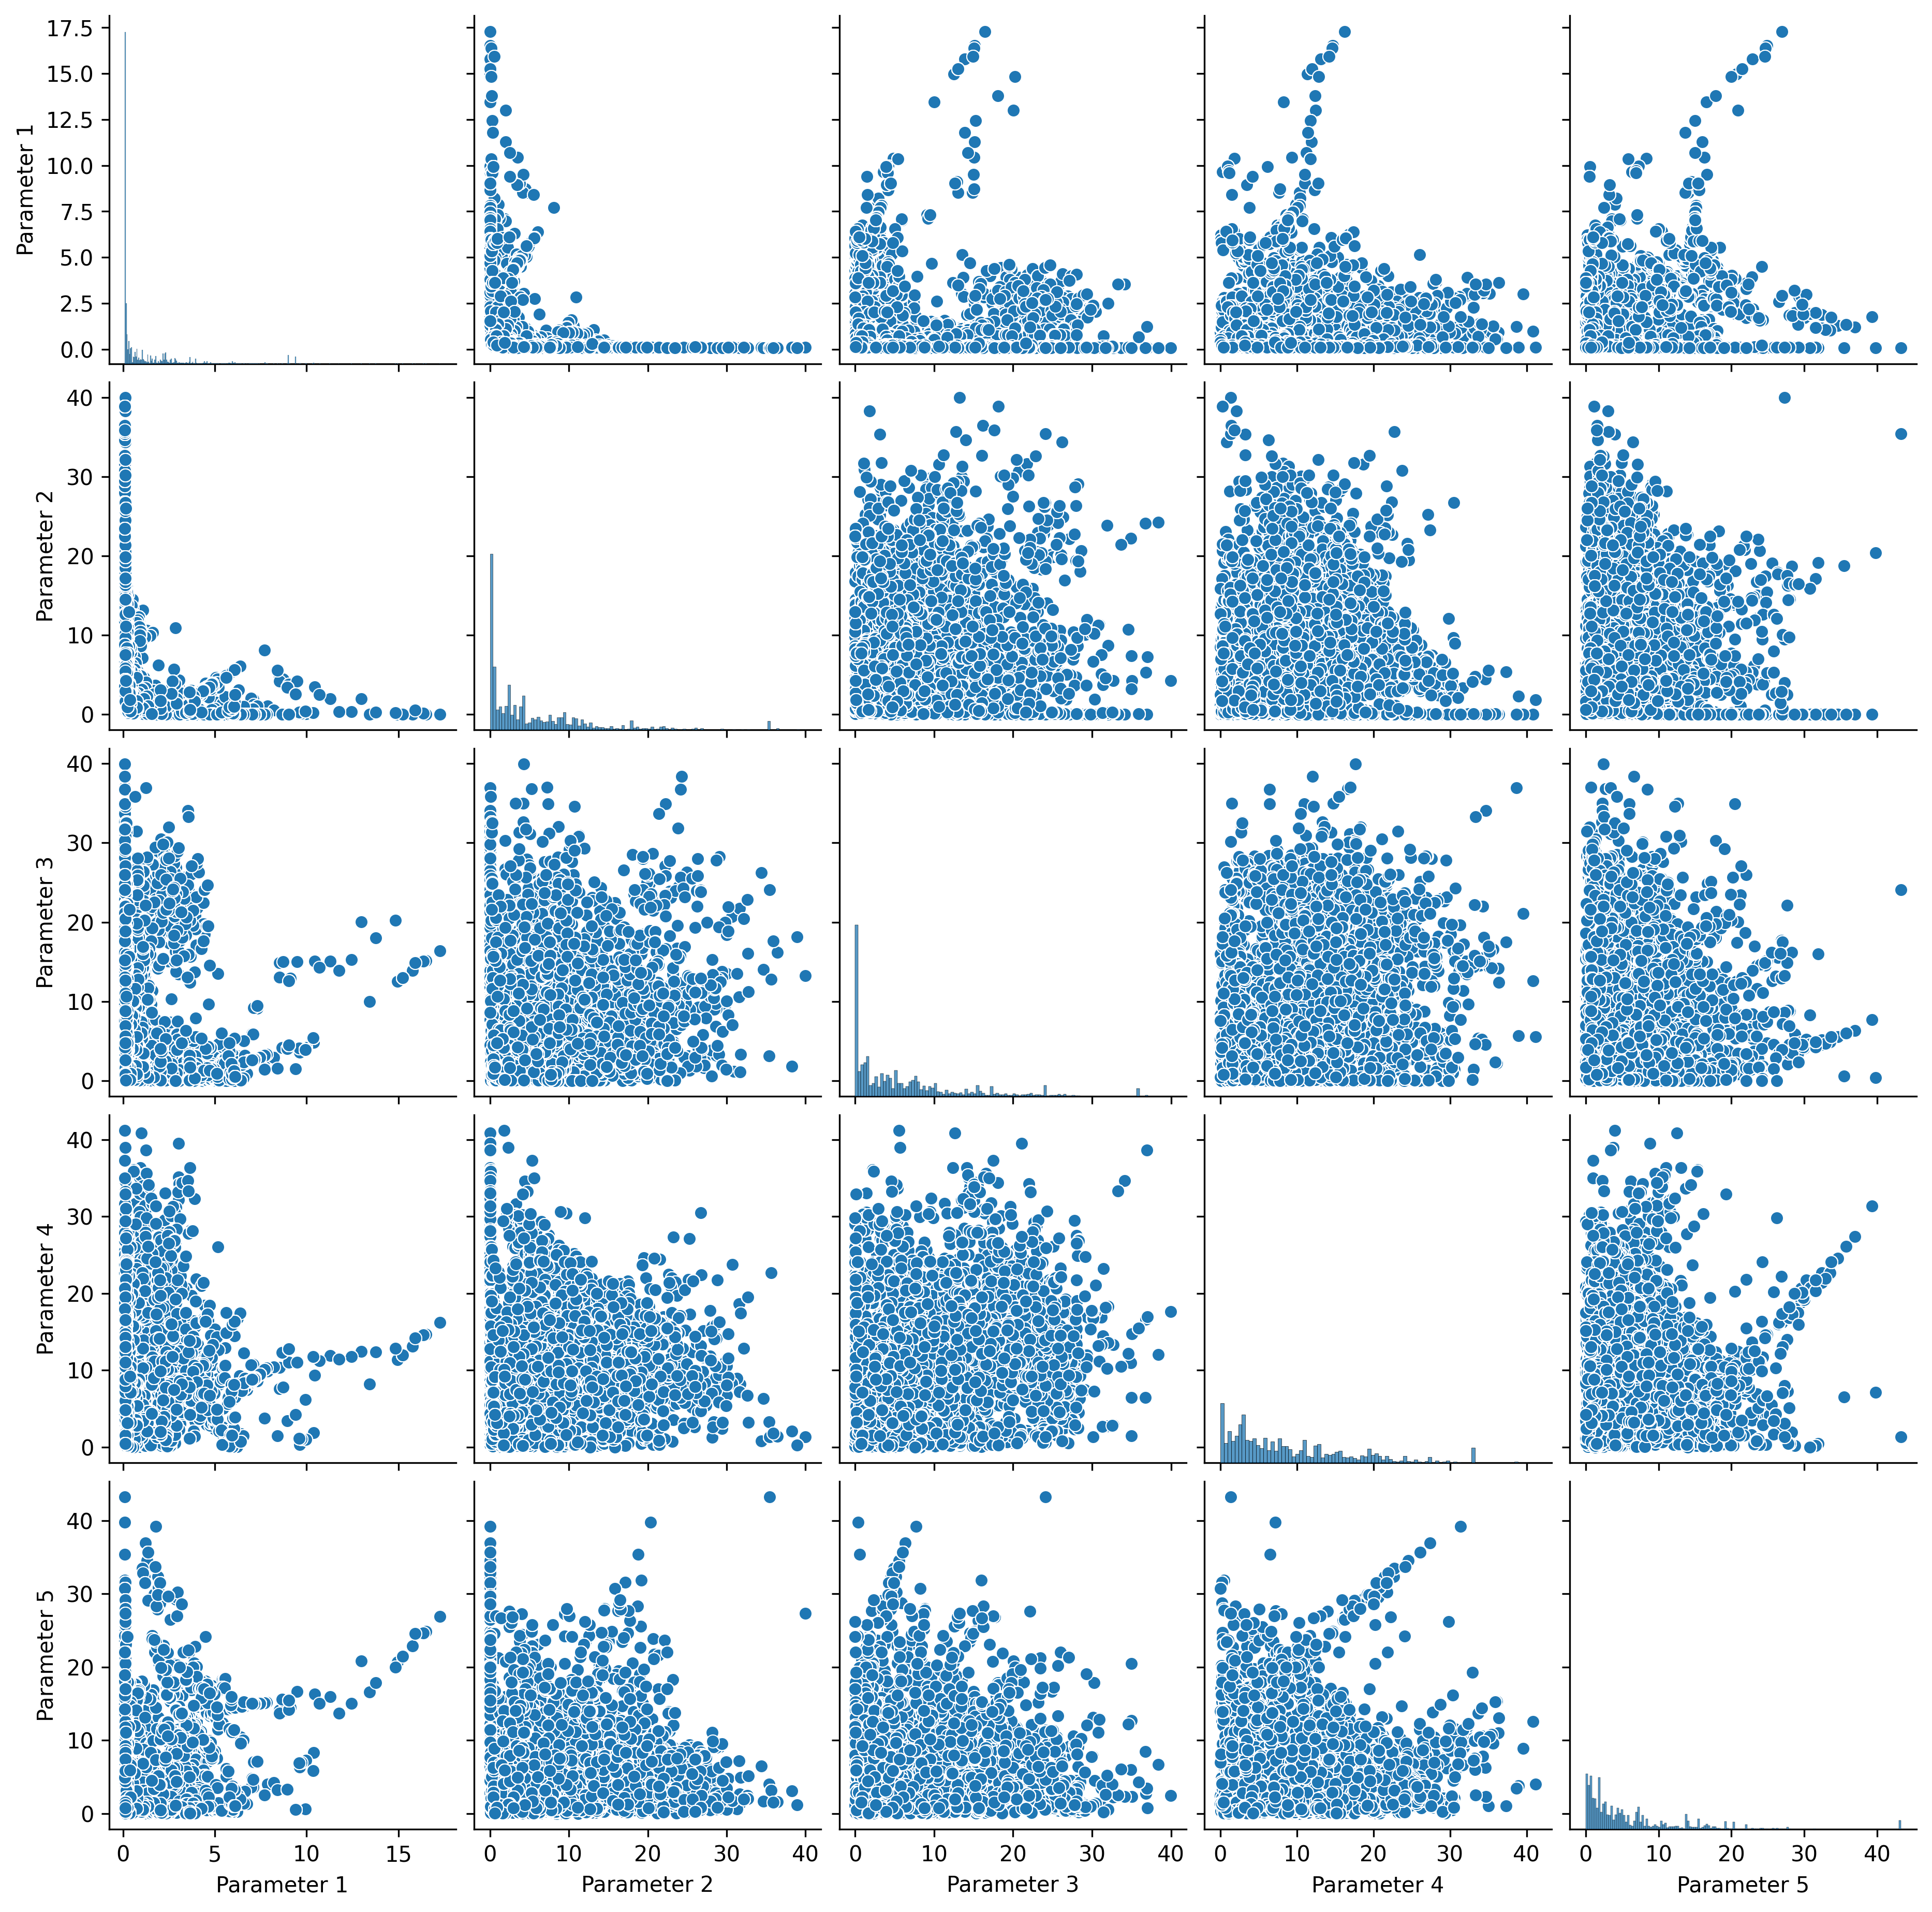
\includegraphics[width=\textwidth]{Figures/appendix_figs/C1.4 pair plot Model 4.png}
\caption{A pair plot of the parameters ($\sigma$) of Model 4. All chains of all ensembles of all samplers (Stretch, DE and DEsnooker) were used to create this figure. Darker shades indicate areas of higher posterior density.}\label{fig_logbook_1.4_pair_model4}
\end{figure}

\subsubsection{check added noise}\label{check noise}
Measurement noise ($\epsilon$) was added artificially to the true hydraulic head values of each cell of the respective MODFLOW models, by sampling from a normal distribution. It was intended that $\epsilon \sim \mathcal{N}(0, 0.1)$. However, it appears that the noise of the observations used for the calibration exercise above, is actually distributed as: $\epsilon \sim \mathcal{N}(0, 0.2)$. This was concluded from computing the mean and standard deviation of the noise, in addition to performing a Shapiro-Wilk test (a test for normality). The Shapiro-Wilk test produced a p-value of 0.74, suggesting $\epsilon$ is Gaussian. Unfortunately, the code for generating this (faulty) noise could not be retrieved. 

The unintentionally large measurement noise is expected to have resulted in the emergence of new optima, different from the true optima. 
%\clearpage at line 224 for placing tables in correct position